%% ----------------------------------------------------------------
%% Thesis.tex -- MAIN FILE (the one that you compile with LaTeX)
%% ---------------------------------------------------------------- 

% Set up the document
\documentclass[a4paper, 14pt, oneside]{Thesis}  % Use the "Thesis" style, based on the ECS Thesis style by Steve Gunn
%\usepackage{graphics}
%\graphicspath{/home/artsiom-bryksa/Bachelor_thesis/Bachelor_thesis/Data}  % Location of the graphics files (set up for graphics to be in PDF format)
% Include any extra LaTeX packages required
\usepackage[square, numbers, comma, sort&compress]{natbib}  % Use the "Natbib" style for the references in the Bibliography
\usepackage{verbatim}  % Needed for the "comment" environment to make LaTeX comments
\usepackage{vector}  % Allows "\bvec{}" and "\buvec{}" for "blackboard" style bold vectors in maths
\usepackage{indentfirst} % To enable indent of the first paragraph in chapter/section
\hypersetup{urlcolor=blue, colorlinks=true}  % Colours hyperlinks in blue, but this can be distracting if there are many links.

\setlength{\parindent}{2em}
\setlength{\parskip}{0em}

%% ----------------------------------------------------------------
\begin{document}

% Set up the Title Page
\title  {Automation of CMS Phase II Tracker Module assembly}
\authors  {\texorpdfstring
            {\href{https://www.linkedin.com/in/artsiom-bryksa-619221121/}{Artsiom Bryksa}}
            {Artsiom Bryksa}
            }
\addresses  {\groupname\\\deptname\\\univname}  % Do not change this here, instead these must be set in the "Thesis.cls" file, please look through it instead
\date       {\today}
\subject    {}
\keywords   {}

\maketitle
%% ----------------------------------------------------------------
{
\setstretch{1.2}  % It is better to have smaller font and larger line spacing than the other way round

% Define the page headers using the FancyHdr package and set up for one-sided printing
\fancyhead{}  % Clears all page headers and footers
\rhead{\thepage}  % Sets the right side header to show the page number
\lhead{}  % Clears the left side page header

\pagestyle{fancy}  % Finally, use the "fancy" page style to implement the FancyHdr headers
}

%% ----------------------------------------------------------------
% Declaration Page required for the Thesis, your institution may give you a different text to place here
\iffalse
\Declaration{

\addtocontents{toc}{\vspace{1em}}  % Add a gap in the Contents, for aesthetics

I, AUTHOR NAME, declare that this thesis titled, `THESIS TITLE' and the work presented in it are my own. I confirm that:

\begin{itemize} 
\item[\tiny{$\blacksquare$}] This work was done wholly or mainly while in candidature for a research degree at this University.
 
\item[\tiny{$\blacksquare$}] Where any part of this thesis has previously been submitted for a degree or any other qualification at this University or any other institution, this has been clearly stated.
 
\item[\tiny{$\blacksquare$}] Where I have consulted the published work of others, this is always clearly attributed.
 
\item[\tiny{$\blacksquare$}] Where I have quoted from the work of others, the source is always given. With the exception of such quotations, this thesis is entirely my own work.
 
\item[\tiny{$\blacksquare$}] I have acknowledged all main sources of help.
 
\item[\tiny{$\blacksquare$}] Where the thesis is based on work done by myself jointly with others, I have made clear exactly what was done by others and what I have contributed myself.
\\
\end{itemize}
 
 
Signed:\\
\rule[1em]{25em}{0.5pt}  % This prints a line for the signature
 
Date:\\
\rule[1em]{25em}{0.5pt}  % This prints a line to write the date
}
\clearpage  % Declaration ended, now start a new page

\fi
%% ----------------------------------------------------------------
% The "Funny Quote Page"
\iffalse
\pagestyle{empty}  % No headers or footers for the following pages

\null\vfill
% Now comes the "Funny Quote", written in italics
\textit{``Write a funny quote here.''}

\begin{flushright}
If the quote is taken from someone, their name goes here
\end{flushright}

\vfill\vfill\vfill\vfill\vfill\vfill\null
\clearpage  % Funny Quote page ended, start a new page
\fi
%% ----------------------------------------------------------------

% The Abstract Page
\addtotoc{Abstract}  % Add the "Abstract" page entry to the Contents
\abstract{
\addtocontents{toc}{\vspace{1em}}  % Add a gap in the Contents, for aesthetics

The CMS phase II upgrade outer tracker is built from two types of modules (PS and 2S) each consisting of two silicon sensors and associated electronics and mechanics. In the case of the PS module, the sensors has be assembled to a precision of approximately 40 mm. In order to satisfy this requirement and a short module assembly time, an automated assembly system is proposed. This systems based on a high-precision motion-stage integrated with high-resolution camera, which provides pattern-recognition, vacuum holding system and control systems. \cite{Reference1}

}

\clearpage  % Abstract ended, start a new page
%% ----------------------------------------------------------------
{
\setstretch{1.2}  % Reset the line-spacing to 1.3 for body text (if it has changed)

% The Acknowledgements page, for thanking everyone
\acknowledgements{
\addtocontents{toc}{\vspace{1em}}  % Add a gap in the Contents, for aesthetics

James Keaveney, Andreas Mussgiller, Doris Eckstein, Carsten Muhl, Adam Zuber and all the CMS group in DESY for being ready to help anytime I had questions, while I had lots of them\ldots

}
\clearpage  % End of the Acknowledgements
}
%% ----------------------------------------------------------------

\pagestyle{fancy}  %The page style headers have been "empty" all this time, now use the "fancy" headers as defined before to bring them back


%% ----------------------------------------------------------------
\lhead{\emph{Contents}}  % Set the left side page header to "Contents"
\tableofcontents  % Write out the Table of Contents

%% ----------------------------------------------------------------
\iffalse
\lhead{\emph{List of Figures}}  % Set the left side page header to "List if Figures"
\listoffigures  % Write out the List of Figures
\fi
%% ----------------------------------------------------------------
\iffalse
\lhead{\emph{List of Tables}}  % Set the left side page header to "List of Tables"
\listoftables  % Write out the List of Tables
\fi
%% ----------------------------------------------------------------
{
\setstretch{1.5}  % Set the line spacing to 1.5, this makes the following tables easier to read
\clearpage  % Start a new page
\lhead{\emph{Abbreviations}}  % Set the left side page header to "Abbreviations"
\listofsymbols{ll}  % Include a list of Abbreviations (a table of two columns)
{
\textbf{CMS} & \textbf{C}ompact \textbf{M}uon \textbf{S}olenoid \\
\textbf{LHC} & \textbf{L}arge \textbf{H}adron \textbf{C}ollider \\
...

}
}

%% ----------------------------------------------------------------
\iffalse
\clearpage  % Start a new page
\lhead{\emph{Physical Constants}}  % Set the left side page header to "Physical Constants"
\listofconstants{lrcl}  % Include a list of Physical Constants (a four column table)
{
% Constant Name & Symbol & = & Constant Value (with units) \\
Speed of Light & $c$ & $=$ & $2.997\ 924\ 58\times10^{8}\ \mbox{ms}^{-\mbox{s}}$ (exact)\\

}
\fi
%% ----------------------------------------------------------------
\iffalse
\clearpage  %Start a new page
\lhead{\emph{Symbols}}  % Set the left side page header to "Symbols"
\listofnomenclature{lll}  % Include a list of Symbols (a three column table)
{
% symbol & name & unit \\
$a$ & distance & m \\
$P$ & power & W (Js$^{-1}$) \\
& & \\ % Gap to separate the Roman symbols from the Greek
$\omega$ & angular frequency & rads$^{-1}$ \\
}
\fi
%% ----------------------------------------------------------------
% End of the pre-able, contents and lists of things
% Begin the Dedication page
\iffalse

\setstretch{0.5}  % Return the line spacing back to 1.3

\pagestyle{empty}  % Page style needs to be empty for this page
\dedicatory{For/Dedicated to/To my\ldots}

\addtocontents{toc}{\vspace{2em}}  % Add a gap in the Contents, for aesthetics
\fi

%% ----------------------------------------------------------------
\mainmatter	  % Begin normal, numeric (1,2,3...) page numbering
\pagestyle{fancy}  % Return the page headers back to the "fancy" style

% Include the chapters of the thesis, as separate files
% Just uncomment the lines as you write the chapters

\chapter{Introduction}


The Large Hadron Collider (LHC) is the largest particle accelerator in the world. During the first run of it from 2010 to 2013 its experiments had made remarkable achievements. Perhaps one of the most famous is the discovery of the theorised Higgs particle, which resulted in the Nobel Prize in Physics in 2013 being awarded to François Englert and Peter Higgs. The LHC are made to collide particles at four locations around the accelerator ring, corresponding to the positions of four particle detectors – ATLAS, CMS, ALICE and LHCb \cite{ref_cern_home}.


\section{Compact Muon Solenoid}


The Compact Muon Solenoid (CMS) is a cylindrical particle detector designed to measure a wide range of particles produced in the collisions of LHC. The size of the detector is around 28 m long and 15 m in diameter. It is the heaviest detector in the world and weighs approximately 14000 t. The name "CMS" originates from the three key characteristics of the detector: its relatively compact size, its excellent capabilities in the detection and measurement of muons and its central feature, a superconducting 3.8T solenoid magnet.

The CMS detector consists of many separate detector layers, each of them playing an individual role in detecting and measuring the traversing particles. A cross-sectional overview of the layers and its tasks in reconstructing tracks of particles is shown in the Figure \ref{fig:cms_layers}.

\begin{figure}[ht]\centering
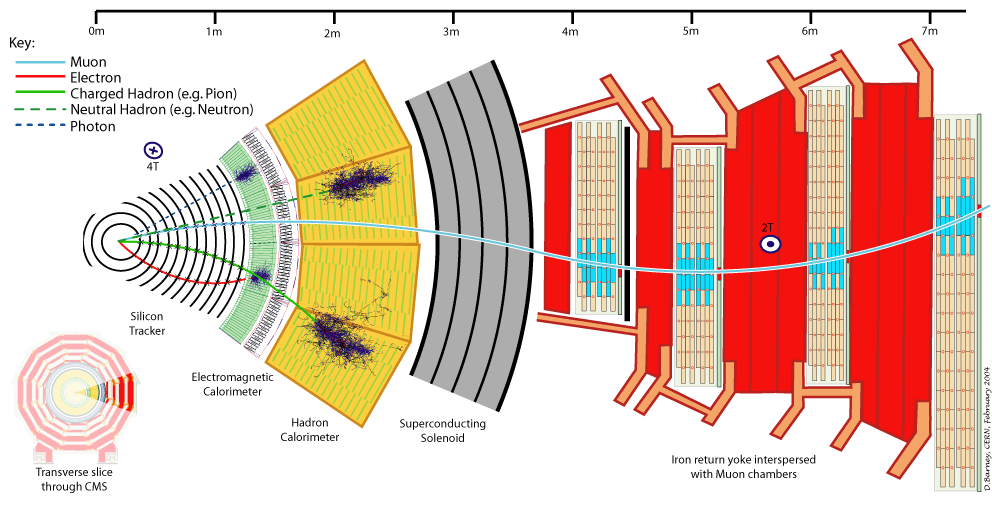
\includegraphics[width=0.8\linewidth]{Data/CMS_layers.png}
\caption{A cross-sectional view of the CMS detection layers.}
\label{fig:cms_layers}
\end{figure}

\section{Phase II Upgrade of CMS Tracker}


After Phase II Upgrade, the LHC will provide a much higher luminosity. This regime is known as the High Luminosity LHC (HL-LHC). A serious problem presented by these conditions is the enormous data readout rates that exceed far beyond the bandwidth foreseen for the readout electronics [2].
However, the vast majority particles produced in the HL-LHC conditions are not of direct interest for new physics searches and are characterized by low transverse momentum. Thus rejecting tracker “hits” related to low transverse momentum particles can significantly reduce the amount of data to be readout. In order to provide momentum discrimination at the hardware level, a 2-layer module design was created. The central idea of the new modules is to provide fast discrimination between low and high momentum particles by estimating the track curvature caused by the magnetic field within the volume of the module itself. For example, particle with high transverse momentum after hitting some pixel/strip at the first sensor layer would hit on of neighboring pixels/strips of the respective pixel/strip on the second layer. While a particle with low transverse momentum would have a more curved trajectory an hit pixel/strips at a displaced position from the first hit. By varying the distance between sensors and number of neighboring pixel/strips required to match hits in adjacent sensors, (2 neighboring strips in the Figure \ref{fig:low_high_pT}) it is possible to set the transverse momentum threshold for a hit~\cite{CMS_TECH_PHASE_II}.


\begin{figure}[ht]\centering
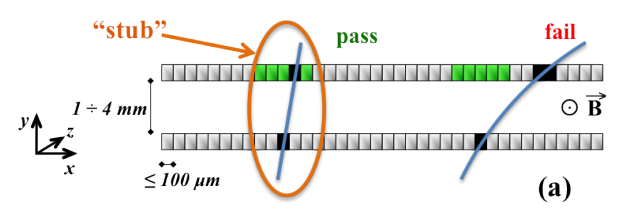
\includegraphics[width=0.8\linewidth]{Data/Introduction/Low_high_pT.png}
\caption{An example of distinguishing high and low transverse momentum. Particles, which hit any of two neighboring strips or the respective strip itself, would be record as high transverse momentum particles.}
\label{fig:low_high_pT}
\end{figure}


\subsection{Two layer Modules}

The CMS Phase-II Tracker will utilize two types of modules, 2S modules and PS modules. To achieve efficient rejection of low-pT particles throughout the Tracker volume, modules in different regions will make use of a few different sensor spacings. For 2S (PS) modules, spacings of 1.8 and 4 mm (1.6, 2.6 and 4 mm) are foreseen. These modules will be used in the end-cap disks as well as the central barrel region of the Tracker. An exploded view of a PS module is shown in Figure \ref{fig:ps_exploaded}. In the PS module, the sensors are glued to a carbon-fibre reinforced Aluminium (AL-CF) spacers which act as spacers and provide the thermal conductance crucial for the cooling of the module. The two sensors and spacers are in turn glued the carbon-fibre (CF) baseplate. This structure is henceforth referred to as the sensor-spacer-baseplate-assembly (SSBA). This project will focus on the assembly of the SSBA only. The precision requirements of the SSBA are shown in figure ??. For the PS module, the sensors must align to within 40 mm measured at the sensor’s short edge. This corresponds to a rotational alignment tolerance of 0.8 mrad.
\begin{figure}[ht]\centering
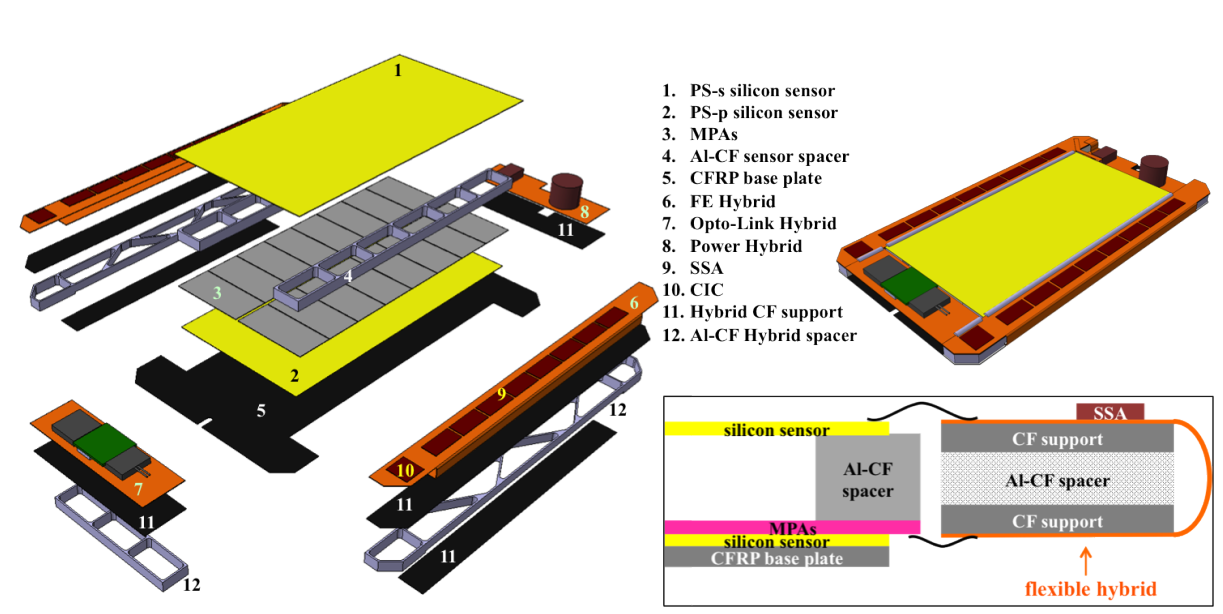
\includegraphics[width=0.8\linewidth]{Data/PS_exploaded.png}
\caption{Exploaded view of Pixesl Sensor Module.}
\label{fig:ps_exploaded}
\end{figure}

\subsection{Assembly of two layer sensors}

 % Introduction

\chapter{Module assembly}

Usual way to assemble such kind of high-precision sensors is a manually assembly with a help of mechanical jig. Alternative way is the proposed automated assembly system.

\section{Manual assembly with mechanical jig}

One option for module assembly is manual assembly with a custom-built mechanical jig (prototype is shown on Figure \ref{fig:mechanical_jig}) \cite{Automated_assembly_slides}.

\begin{figure}[ht]\centering
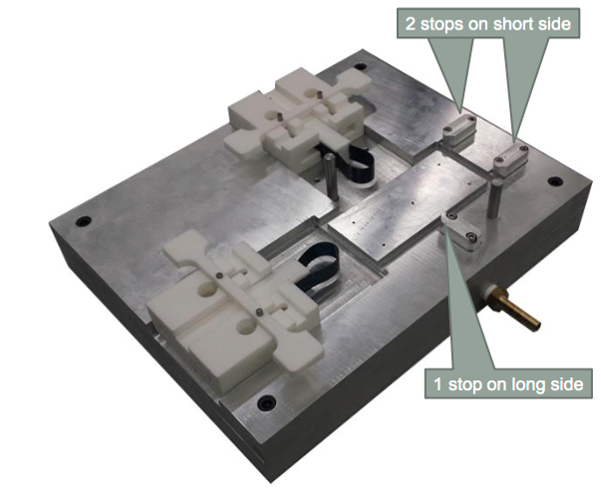
\includegraphics[width=0.7\linewidth]{Data/Module_assembly/Mechanical_jig.png}
\caption{Prototype of the mechanical jig for module assembly.}
\label{fig:mechanical_jig}
\end{figure}

With such method of assembly all parts are placed in the jig and glued together manually. To provide required accuracy mechanical jig has 3 reference stops: one along the longer side of the module and two along the shorter side. From opposite to reference stops sides the module is gently pushed by springs towards reference stops. Together they provide enough precise positioning of the module's components before and during gluing.

However such method of module assembly has a number of disadvantages. It is relatively slow and does not scale well for high number of modules to assemble. In addition, such mechanical system has poor repeatability and has no options to control the process. Moreover, it needs very precise machining technologies (several microns precision) to manufacture this mechanical jig, as well as regular calibration of reference stops positions. Finally, this mechanical system need maximum manual handling and highly depends on human operating it. This fact means that even though in theory system can provide required quality of the assembled modules, there will be always more or less several percentage of modules assembled out of required quality only because of a human mistake.

\section{Automated assembly system}

The proposed automated assembly system consists of three sub-systems: the motion subsystem, the vision subsystem and the vacuum subsystem (Figure \ref{fig:auto_assembly_system})\cite{AutomatedAssembly_tutorial}.

\begin{figure}[ht]\centering
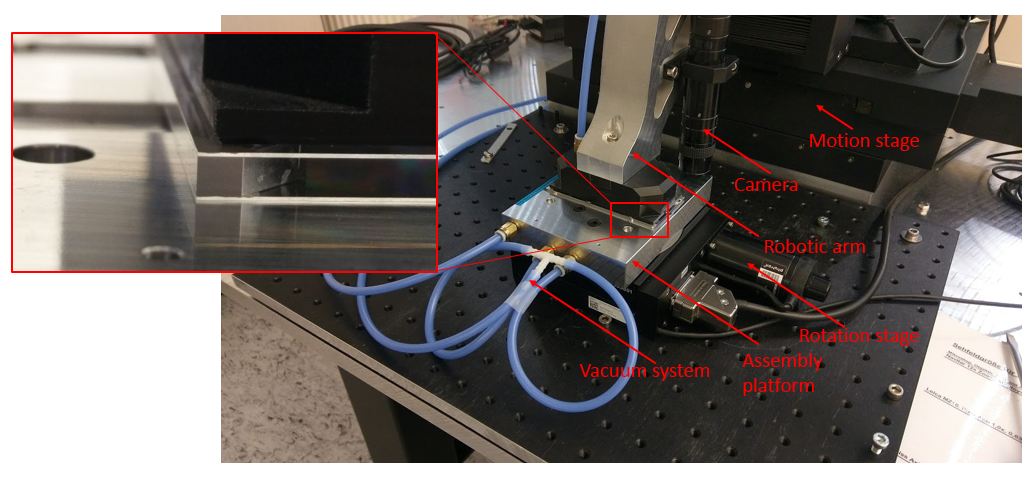
\includegraphics[width=1\linewidth]{Data/Module_assembly/Automated_assembly_system.png}
\caption{Proposed automated assembly system.}
\label{fig:auto_assembly_system}
\end{figure}

The motion system provides the precise mechanical movements needed to arrange the components comprising the SSBA. Movement of the components is achieved via mounting on the two moveable parts of the motion system: the x-y-z and rotation stages. An custom-built AL tool known as the arm is mounted on the x-y-z stage allowing mounting of components and thus movement of components in Cartesian coordinates. Components placed on the rotation stage may rotate in the horizontal plane with an angle $\theta$. The motion stages are controlled by a motion controller unit. All motion hardware is manufactured by Lang 1 with motion precisions of 4~um and 2~mrad respectively. The vacuum system enables the mounting of components to the arm and rotation stage. It consists of a single pump providing vacuum to four switchable valves which in turn distribute vacuum to independent vacuum lines. The valves are switched to on(off) states by applying a control signal of 12~(0)V. The 12V signals are provided by a relay card. One vacuum line connects to the a pickup tool which is mounted on the arm, others -- to the assembly platform. The pickup tool consists of an ESD plastic block housing an inner vacuum chamber which distributed the vacuum to an array of downward facing suction cups which slightly protrude below the bottom side of the tool. A diagram of the pickup tool is shown in Figure \ref{fig:pick_up_tool}.

\begin{figure}[ht]\centering
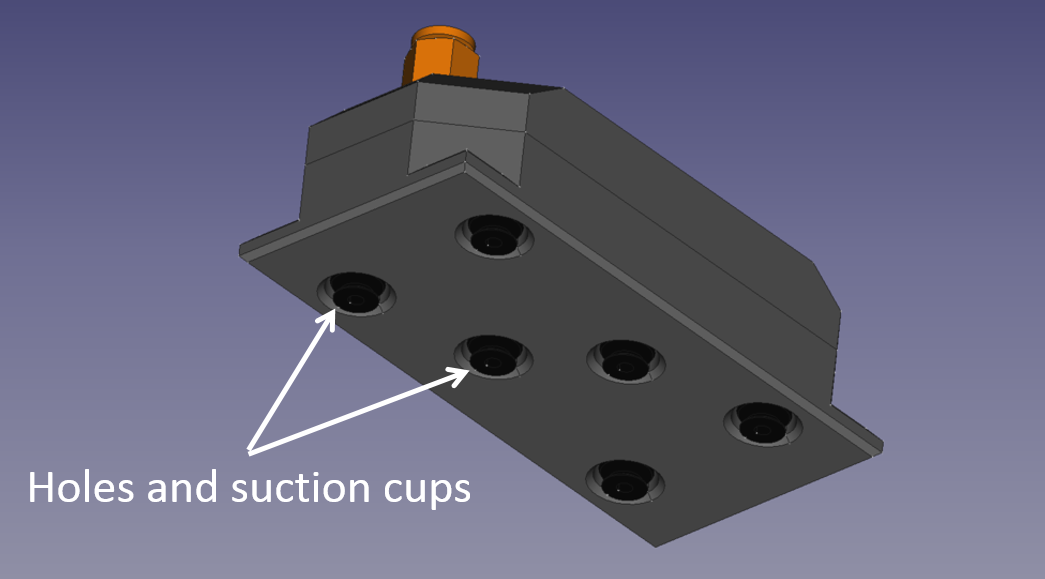
\includegraphics[width=0.7\linewidth]{Data/Module_assembly/Pick_up_tool.png}
\caption{Pick-up tool.}
\label{fig:pick_up_tool}
\end{figure}

The pickup procedure is performed by contacting the suction cups with the sensor, switching on the vacuum within the pickup tool and moving the arm directly upwards with the sensor attached. The setdown procedure is performed by contacting the mounted sensor (or baseplate) with the lower surface on which the component will be placed, switching off the vacuum in the pickup tool and moving the arm away. In order to avoid any movement of the component as the arm moves away, the component will be fixed in its setdown position with a separate array of upward-facing suction cups and independent vacuum line. The vision system acquires images of components allow determination of their positions and orientations which is crucial for precise assembly.

The vision system consists is represented by high-resolution camera by IDS. The camera is mounted on the arm and is referred to as the mobile camera. It is fixed in a downward-facing orientation. The camera acquires images immediately before pickups and immediately after setdowns in order to determine the positions of unmounted components. 

\section{Assembly platform}

One of the very important part of the automated assembly system is an assembly platform. the main purpose of it is to fix module components underneath with a vacuum.

The assembly platform should fulfil the following requirements:

\begin{enumerate}
\setlength\itemsep{-0.5em}
\item Fix all necessary module components with vacuum on top of the platform.
\item Provide the possibility of precise placement and orientation for two spacers.
\item To be reasonably light and have center of mass close to the rotation axis of a rotation stage it will be attached to.
\end{enumerate}

In order to match above mentioned requirements, the following design was proposed (Figure \ref{fig:platform_design}):

\begin{figure}[ht]\centering
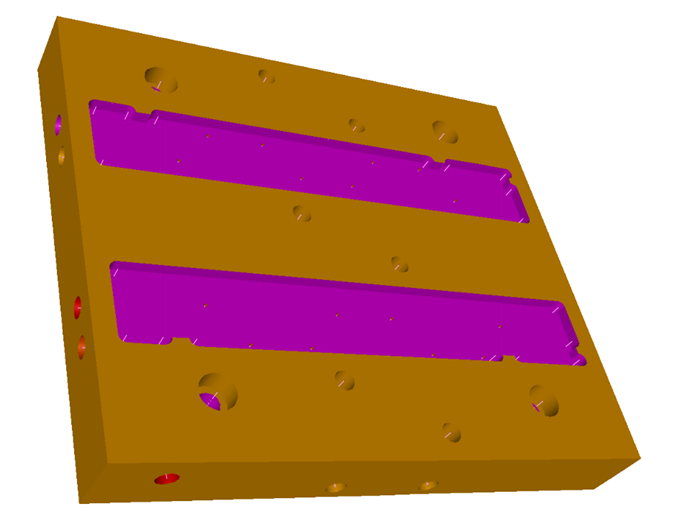
\includegraphics[width=0.7\linewidth]{Data/Module_assembly/Platform_design.png}
\caption{Design of the assembly platform.}
\label{fig:platform_design}
\end{figure}

Assembly platform has two inserts with three reference stops each to provide precise placement of spacers. Comparing to mechanical jig, assembly platform's reference stops are part of the platform itself and do not need a calibration. However having such inserts makes direct placement of the other flat components (sensors, baseplate) on top of the inserts impossible, because major area of them would have lack of underneath support under the pressure of pickup tool on top while glue curing. To solve this problem it was decided to place these components on the assembly platform perpendicular to spacers. In this case only a small area of components would have no support underneath, which is fine for assembly tasks. Perpendicular components placement on the assembly platform can be easily provided by rotation stage the platform mounted on. The platform center of mass is very close to the rotation axis (less than 1~mm) and its weight is around 1~kg thus there will no negative effects on the precision of the rotation stage operations. 

The assembly platform houses two independent inner vacuum chambers: the first for spacers holding, the second for holding other flat module components. The chamber for spacers' vacuum system distributes vacuum into the array of tiny holes (0.7~mm in diameter) on the bottom of the inserts. The size and placement of these vacuum holes is determined by the shape of spacers (Figure \ref{fig:al_spacer}). These holes do not equipped with a suction cups due to such tiny size. So small suction cups simply do not exist in the market. Additionally, the flatness of contiguous surfaces (inserts bottom and spacer) cause relatively small vacuum leakage thus providing enough tight vacuum fix of the spacers.

\begin{figure}[ht]\centering
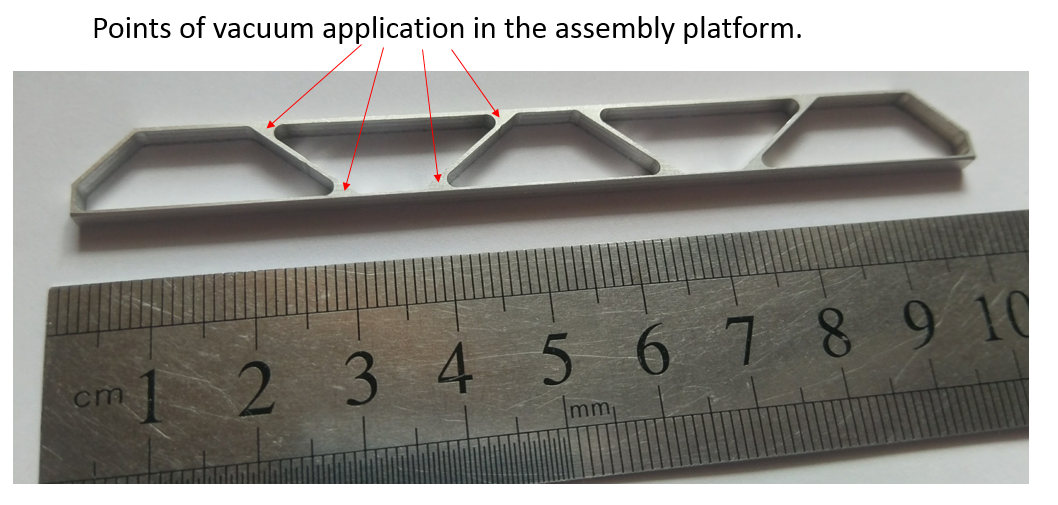
\includegraphics[width=0.7\linewidth]{Data/Module_assembly/Al_spacer.png}
\caption{Al spacer for the PS module.}
\label{fig:al_spacer}
\end{figure}

The second vacuum chamber distributes the vacuum in the array of suction cups to hold other flat module components (sensors and baseplate). It uses the same suction cups as pickup tool. Just as in the pick up tool, they stitch out a bit form the surface of the assembly platform. However, they should not prevent gluing components to spacers, stored in the inserts. That is why the depth of the interests is less than the thickness of spacers thus upper surface of the spacers stored in the inserts is a bit higher than suction cups. In other words, suction cups do not prevent operating with spacers as soon as they are lower, than upper surface of the spacers.

\section{Fast curing adhesive}

One of the crucial part of the automated assembly system is an adhesive using in the assembly, to be more  -- its curing time. Otherwise it makes a few sense to leave one module for a long time in the whole setup simply waiting the adhesive curing time. For instance, current guideline glue takes 24 hours to cure. That is why automated assembly needs a technique to avoid such long waiting. One of the proposed decision is using a small amount of fast curing adhesive in addition to main guideline glue. This adhesive should fulfil the following requirements:

\begin{enumerate}
\setlength\itemsep{-0.5em}
\item Provide reasonable bond after about 15 minutes.
\item Have no interference with main adhesive.
\item Have a thin layer (approximately less than 30~um).
\end{enumerate}

Moreover, mentioned above requirements should be completed with as small amount of fast curing adhesive as possible. For gluing tests we used simple rectangular shape Al samples (representing Al-CF spacers) and glass samples (representing Silicon sensors). Reaching listed requirements highly depends on two aspects: first -- the way fast adhesive is applied, second -- fast adhesive properties.

There are lots of possible way of applying fast adhesive: several fast adhesive drops inside main adhesive layer, several drops close to edges, bevel gluing (fill the bevel space of the Al sample with fast adhesive), side gluing (put some fast adhesive on sides), etc. For our system we decided to test bevel gluing and fast adhesive drops close to the edge. Even though bevel gluing can provide reasonable bond after 15 minutes, it is way more handy to use just two fast adhesive drops close to the edge. Adhesive was applied as shown on the Figure \ref{fig:glue_application}. 

\begin{figure}[ht]\centering
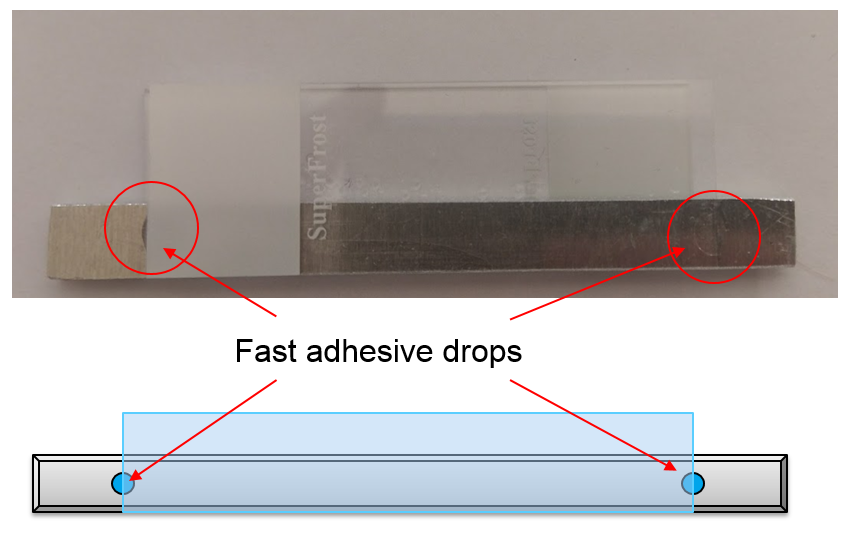
\includegraphics[width=0.7\linewidth]{Data/Module_assembly/Fast_glue_application.png}
\caption{The way of fast adhesive application during glue tests. Much smaller drops can be used for obtaining reasonable bond.}
\label{fig:glue_application}
\end{figure}

The second part of the part of the question -- finding proper fast adhesive in the market. The main issue of this question is combining two following properties: fast curing and low viscosity. Low viscosity is an integral property of the adhesive in case it should provide thin glue layer. However, fast curing means that adhesive must become hard quickly which is easier when it is initially has high viscosity. That is reason it is hard to find an adhesive combining both these properties. Nevertheless, there were several candidates for tests:

\begin{enumerate}
\setlength\itemsep{-0.5em}
\item \textit{Polytec EP 660}. According to the datasheet \cite{Polytec_EP_660_datasheet}, its curing time is about 16 hours which is too far beyond the requirements. However, the distributor said it worth trying as soon as 16 hours in a full curing time and so called handling time is shorter. Unfortunately, it this adhesive did not provide any bond after 15 minutes, as expected. The only advantage of this adhesive is that it is the same vendor as main guideline adhesive what could probably results in some financial benefits.
\item \textit{Loxeal 31-42}. According to the datasheet \cite{Loxeal_31_42_datasheet}, its full curing time is 20-30 minutes, while handling time is around 3-8 minutes. As a result it successfully provided reasonable bond after 15 minutes.
\item \textit{Wekem WK5}. According to the datasheet \cite{Wekem_WK_5_datasheet}, its curing time is around 5 minutes. It also provided reasonable bond after 15 minutes, but Loxeal adhesive has better quality and easier to operate with. Moreover, Loxeal glue provide thinner glue layer under the same pressure while curing: $<~20~um$ while Wekem provides around 40~um (Figure \ref{fig:glue_thickness}).
\end{enumerate}

\begin{figure}[ht]\centering
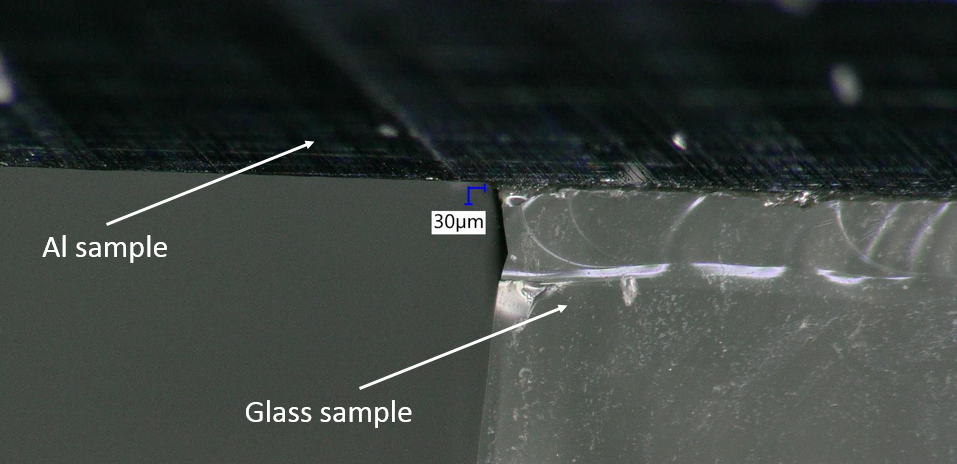
\includegraphics[width=0.7\linewidth]{Data/Module_assembly/Loxeal_393g_point_1.png}
\caption{Glue layer thickness of Loxeal~31-42 under the pressure of around $20~g/cm^{2}$}
\label{fig:glue_thickness}
\end{figure}

Talking about interaction with the main guideline adhesive, a series of test was done to check this property of the Loxeal 31-42. Among them were:

\begin{enumerate}
\setlength\itemsep{-0.5em}
\item \textit{Gluing test of two drops of fast and main adhesive in touch.} Tightness of glue bond remained approximately the same after 15 minutes curing comparing to separate fast gluing test.
\item \textit{Gluing test of two mixed drops of fast and main adhesive.} Tightness of glue bond slightly decreased after 15 minutes curing comparing to separate fast gluing test.
\end{enumerate}

To conclude, Loxeal fast adhesive clearly showed better qualities among other adhesives and fulfil all the requirements: it provides reasonable bond after 15 minutes and light pressure (around $20~g/cm^{2}$), has thin glue layer -- $<~20~um$ and show no interaction with the main guideline adhesive (touching the main adhesive).

\section{Automated assembly process}

Automated assembly process of a PS module consists of following steps:

\begin{enumerate}
\setlength\itemsep{-0.5em}
\item \emph{Prepare top sensor.} Firstly, put manually the top sensor to the platform and fix it with the vacuum. Next, detect its location and orientation with a help of camera and special software and save the data. Correct the orientation of the sensor with a help of rotation stage so thus it will be parallel to the X-axis of the motion stage. Finally, pick it up with the pickup tool and leave it attached to it. The vacuum on the pick up tool will remain applied during the whole assembly process beginning from this very first step.
\item \emph{Prepare spacers.} Once the top sensor removed from the platform and attached to the pickup tool, the platform should rotate by 90~degrees so that spacers can take their spots with the correct orientation relatively to the top sensor. Next, gently pushed to the reference stops and got fixed with the vacuum from the platform. Then the system should find and locate the reference marker on the platform thus being able to deduce the location of the spacers.
\item \emph{Glue top sensor to spacers.} Once both top sensor and spacers are ready and their locations are identified, the software can easily calculated the path for the pickup tool with attached top sensor on it. Next is to put the main adhesive and several drops of the fast adhesive on the spacers and move the pickup tool to the calculated gluing position. Special attention should be paid for Z coordinates of pickup tool moving as soon as it directly influence the thickness of the glue layer.
\item \emph{Prepare bottom sensor.} After about 15~minutes the fast adhesive drops are cured and provide reasonable bond to remove just glued spacers with top sensor. To do this pickup tool should simply move upwards with vacuum remaining applied. After the platform is cleared it should rotate by 90~degrees so that the bottom sensor can be placed and fixed with the vacuum. Next, just as for top sensor, detect its location and orientation with a help of camera and special software and save the data. Correct the orientation of the sensor with a help of rotation stage so thus it will be parallel to the X-axis of the motion stage which means parallel to the top sensor.
\item \emph{Glue bottom sensor to spacers~+~top~sensor.} All the required components for this step are fixed and theirs locations are identified. Hence the software is able to calculate the path for the pickup tool. Finally, pickup tool can move to the gluing position after applying main and fast adhesives.
\item \emph{Prepare baseplate.} After about 15-minutes glued structure can be lifted up with the pick up tool and its vacuum still remaining applied. Next is placing the baseplate paying attention for three reference pins and fix it with vacuum. These pins are not exist in the current version of the assembly platform as soon as gluing baseplate to the sensor-spacers-sensor (bare module) is not a high priority for the current state of the project. The reason for that -- baseplate gluing do not required so high accuracy as bare module.
\item \emph{Glue sensor-spacers-sensor structure (bare module) to the baseplate.} As soon as the software has already known the position of the reference marker on the assembly platform, hence it is able to calculate the location of the baseplate and the gluing position of the pickup tool with bare module attached to it. Finally, the pickup tool moves to the gluing position after applying main and fast adhesives.
\item \emph{Automated assembly is done.} After about 15 minutes fast adhesive provides enough bond and the assembled module (a part of it to be precise) can be removed from assembly platform and left for 24~hours to let the main adhesive cure. However, baseplate's reference pins fits the baseplate very tight thus manual removing can likely cause break. That is why it is better to remove the module with a pick-up tool as soon as it can provide perpendicular lift which is safer.
\end{enumerate} % Module assembly 

\chapter{Control Software}

In order to control the whole automated assembly system a PC-based Qt~application was developed. All the necessary hardware is connected to the PC with USB interface.

\section{General structure of the application}

The control of the motion, vision and vacuum subsystems is integrated in a single software application henceforth referred to as PSAuto (from automated assembly of PS module). It is entirely written in C++ and utilises the Qt~framework version~4.8.7. A schematic illustrating the integration of the subsystems with PSAuto is shown in Figure \ref{fig:general_app_structure}.

\begin{figure}[ht]\centering
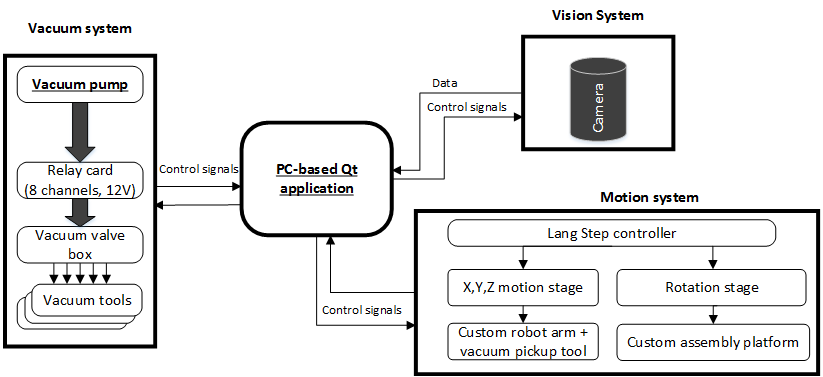
\includegraphics[width=1\linewidth]{Data/Control_Software/Whole_system_diagram_(English).png}
\caption{A schematic view of the integration of the motion, vision and vacuum subsytems via the Qt-application.}
\label{fig:general_app_structure}
\end{figure}



\subsection{Model View Controller architectural pattern}

The architecture of the application is based on Model-View-Controller (MVC) architectural pattern. It considers there to be three main types of objects: \emph{model} objects, \emph{view} objects and \emph{controller} objects. When designing an application, a major step is choosing or creating custom classes for objects that fall into one of these three groups. Each of the three types of objects is separated from the others by abstract boundaries and communicates with objects of the other types across those boundaries. The pattern defines not only the roles objects play in the application, it also defines the way objects communicate with each other \cite{apple_MVC}. The key point of MVC is that View and Controller depend on Model, but Model does not depend on them. The  interaction of these three types is schematically shown in the Figure \ref{fig:mvc_general}.

\begin{figure}[ht]\centering
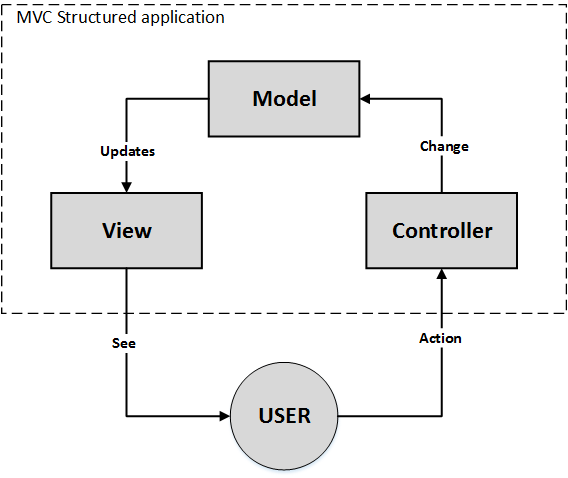
\includegraphics[width=0.7\linewidth]{Data/Control_Software/MVC_general.png}
\caption{Model, View and Controller (MVC) relative to user (classic interaction).}
\label{fig:mvc_general}
\end{figure}

Shown in the Figure \ref{fig:mvc_general} interaction is a classical MVC architecture. There are various realization of this diagram in terms of interaction between three main object types of MVC. The main reasons of it are various application types and their realizations. For instance, in the PSAuto application this diagram will look like in the Figure \ref{fig:mvc_custom}.

\begin{figure}[ht]\centering
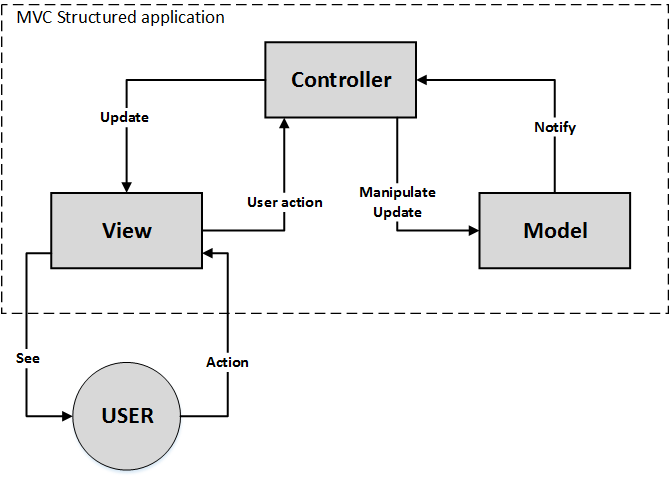
\includegraphics[width=0.7\linewidth]{Data/Control_Software/MVC_custom.png}
\caption{Model, View and Controller (MVC) relative to user (interaction in the PSAuto).}
\label{fig:mvc_custom}
\end{figure}

Comparing to classical MVC structure from Figure \ref{fig:mvc_general}, the Model do not directly inform/update the View. This information passes through Controller. A controller object acts as the intermediary between the Model and the View. Controller is often in charge of making sure the Views have access to the Model objects they need to display and act as the conduit through which views learn about changes to the Model. Controller objects can also perform set-up and coordinating tasks for an application and manage the life cycles of other objects \cite{apple_MVC}.

Depending on the application logic and demands, Model, View and Controller follow special properties and rules.

\emph{Model} is central component of the system. It directly manages the data, defines the logic and rules of the application which manipulates the date. Moreover, like in our case, it regulates the interaction between the application and hardware. For instance, there is a Model class \emph{ConradModel} in PSAuto application. It is responsible for communication with a relay card for turning on and off vacuum lines. This class completely meet MVC rules as a Model object because it does not depend on any other class, while others depend on it using its possibilities for their functions.

\emph{View} unite all objects responsible for visual part of the application: windows, tabs, labels, forms, buttons, etc. They know how to display the data from the application's model and also give a user the possibility to edit the data. For instance, one task of \emph{AssemblyModuleAssembler} class is to display the information about Vacuum lines of the system, as well as control elements for it. However, it only display the control elements, but not process the user's actions.

\emph{Controller} is mainly responsible for accepting input and processing it, generating commands for the Model or the View. For instance, \emph{ConradManager} provides all necessary functions to control the vacuum lines and to get the current status of it. It is worth noting that very often there is no direct connection between the Model and the View, like it is shown in the classical MVC architecture in the Figure \ref{fig:mvc_general}. Instead of it, the Controller acts as the intermediary between the application's model objects and its view objects.

\subsection{OpenCV library}

A lot of algorithms needed for the application were found in the open-source library~---~OpenCV (\textit{Open Source Computer Vision}). It is a cross-platform library of programming functions mainly oriented on real-time computer vision. It was originally developed by Intel's research center in Nizhny Novgorod (Russia). Later it was supported by Willow Garage and is now maintained by Itseez. The library is free for use under the open-source BSD license~\cite{OpenCV_general}.

OpenCV was designed for computational efficiency and, as was already mentioned, with a strong focus on real-time applications. It is written in optimized C++ and can take advantage of multicore processors. There is also a possibility for further automatic optimization on Intel architecture with Intel's \textit{Integrated Performance Primitives (IPP)} libraries, which consist of low-level optimized routines in many different algorithmic areas~\cite{kaehler2016learning}.

One of the main goals of OpenCV is to provide a simple-to-use computer vision infrastructure that helps people build fairly sophisticated vision applications quickly. In its libraries one can find over 500 functions that span many areas in vision. In the list below one can see main features of the OpenCV library~\cite{Illinois_openCV}:
\begin{itemize}
\setlength\itemsep{-0.5em}
\item Image data manipulation (allocation, release, copying, setting, conversion).
\item Image and video I/O (file and camera based input, image/video file output).
\item Matrix and vector manipulation and linear algebra routines (products, solvers, eigenvalues, SVD).
\item Various dynamic data structures (lists, queues, sets, trees, graphs).
\item Basic image processing (filtering, edge detection, corner detection, sampling and interpolation, color conversion, morphological operations, histograms, image pyramids).
\item Structural analysis (connected components, contour processing, distance transform, various moments, template matching, Hough transform, polygonal approximation, line fitting, ellipse fitting, Delaunay triangulation).
\item Camera calibration (finding and tracking calibration patterns, calibration, fundamental matrix estimation, homography estimation, stereo correspondence).
\item Motion analysis (optical flow, motion segmentation, tracking).
\item Object recognition (eigen-methods, HMM).
\item Basic GUI (display image/video, keyboard and mouse handling, scroll-bars).
\item Image labeling (line, conic, polygon, text drawing).
\end{itemize}

The application of the OpenCV libraries will be described more detailed in the next section.

\section{Pattern recognition}

Pattern recognition is a crucial part of the whole automated assembly system, in particular -- vision subsystem. It provides the software with the information where all the components of the modules are situated in the space and theirs orientation. Within this information the software is able to calculate where to move each component of an assembling module \cite{AutomatedAssembly_tutorial}.

An important task performed by PSAuto is the determination the \emph{location} and \emph{planar orientation}. By definition, planar orientation is the rotational orientation of the sensor in the horizontal (X-Y) plane of the sensors during the assembly process. For automated assembly system planar orientation is performed in two basic steps: the independent determination of \emph{localised} positions and orientations of the four markers at the corners of the sensor and a global fit to these positions from which the final position and orientation of the entire sensor is extracted. This is done by processing the images of \emph{fiducial markers} at the corners of the sensors (Figure \ref{fig:fiducial_marker}) acquired by the vision system with a Pattern Recognition algorithm. The markers are precisely positioned with respect to the strips or pixels of the sensors. Hence precise alignment of the markers ensures precise alignment of the pixels or strips. The algorithm takes raw images as input and returns the position and orientation of fiducial markers located at the corners of the PS sensors. The pattern recognition algorithm utilises the \emph{OpenCV} package. The steps comprising the pattern recognition are now outined:

\begin{enumerate}
\setlength\itemsep{-0.5em}
\item Pre-processing of raw image.
\item Determination of positions and planar orientations of fiducial markers.
\item Location of other corners and extraction of final position and orientation.
\end{enumerate}

\begin{figure}[ht]\centering
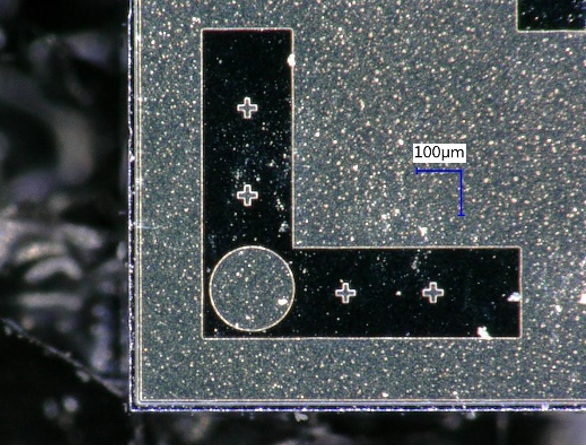
\includegraphics[width=0.7\linewidth]{Data/Control_Software/Fiducial_marker.png}
\caption{Fiducial marker on one of the corner of a PS module's sensor.}
\label{fig:fiducial_marker}
\end{figure}

\subsection{Pre-processing of raw image}
The raw images from the camera are first converted from colour to black and white which is known as \emph{grayscaling} in OpenCV. The pixels comprising the grayscaled image contain intensity information only in the form of a single number ranging from 0 to 255 describing the darkness of a shade of gray as opposed to the intensity and colour information contained in the pixels of a colour image. As the corner markers are based on simple shapes and not colours, the colour information is not helpful and is thus disregarded. The grayscaled image is then converted to a \emph{binary} image in which each pixel is either black or white in a process known as \emph{thresholding}. Thresholding simply converts each pixel of the image into a white(black) pixel if the intensity of the pixel is above(below) a pre-defined threshold. Thresholding serves to reduce the differences between images of identical sensors due to random \emph{noise} arising from dust and random differences in the surfaces of the patterned sensors. Examples of grayscaled and thresholded images of the same corner marker of a dummy PS sensor is shown in Figure \ref{fig:threshold}. The optimal threshold will depend on the ambient lighting conditions around the assembly area and the contrast of the fiducial markings on the sensors. Currently, typical values of threshold are around 90.

\begin{figure}[ht]\centering
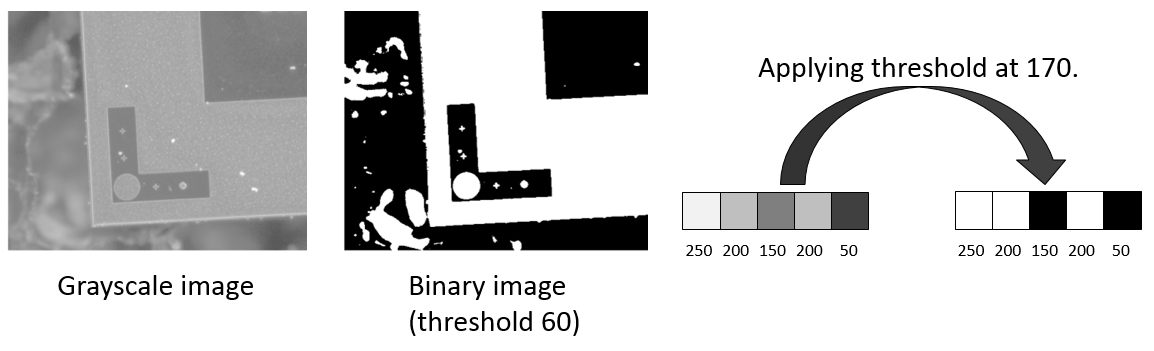
\includegraphics[width=0.9\linewidth]{Data/Control_Software/Threshold.png}
\caption{Threshold application on fiducial marker of dummy PS module's sensor.}
\label{fig:threshold}
\end{figure}

\subsection{Determination of positions and planar orientations of fiducial markers.}
The position and orientation of the fiducial marker within the thresholded image is determined using a standard image processing technique known as \emph{template matching}. OpenCV provides the function of the same name for such kind of tasks. In template matching, parts of an master image that closely resemble a template image are located. In this case, the master image corresponds to the thresholded image of the fiducial marker and the template image corresponds to a thresholded image of a fiducial marker.

Template matching proceeds by iteratively superimposing the template image at each point of the master image and calculating a metric which describes the similarity of the template image and the portion of the master image with which it coincides. The OpenCV package provides multiple options for the metric. Similar results are observed for each possible metric with the chosen metric based on the normalised squared difference between the intensities of coincident pixels of the master image and superimposed template:


\begin{center}
$R(x,y)=\dfrac{\sum_{x',y'}^{}(T(x',y')-I(x+x',y+y'))^{2}}{\sum_{x',y'}^{}\sqrt{\sum_{x',y'}^{}T(x',y')^{2}\cdot\sum_{x',y'}^{}I(x+x',y+y')^{2}}}$
\end{center}
where I denotes \emph{master image}, T -- \emph{template image} and R -- \emph{resultant metric}.

This metric is referred to as CV\_TM\_SQDIFF\_NORMED in OpenCV. The point in the master image where the metric reaches a minimum represents the most probable location of the fiducial marker. In Figure \ref{fig:template_matching} the determination of marker position with template matching and its result using images of the dummy sensor is illustrated. The most probable location of the marker as determined by the algorithm is indicated by the white rectangle. The observed location matches closely with expectation.

\begin{figure}[ht]\centering
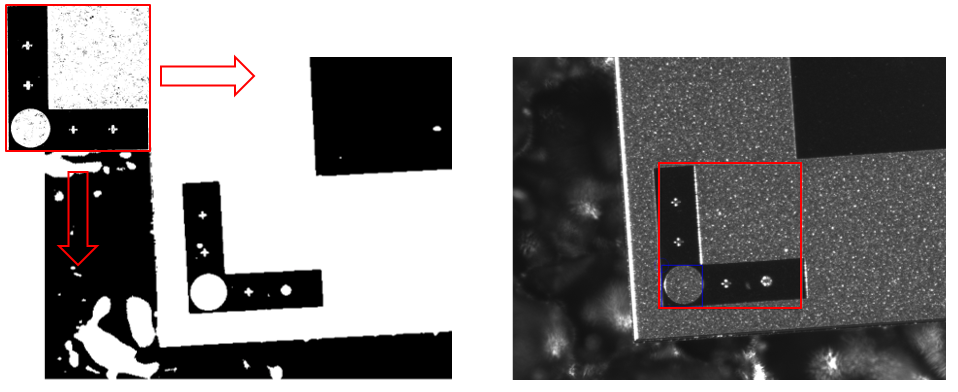
\includegraphics[width=0.9\linewidth]{Data/Control_Software/Template_matching.png}
\caption{The technique of template matching is illustrated on the left image. The red arrows indicate the iterative calculation of a metric at each point of the master image. The result of a template matching routine on using test images is shown on the right image. The most probable location of the marker in the master image is outlined by the red rectangle.}
\label{fig:template_matching}
\end{figure}

In order to deduce the orientation of the marker in the plane transverse to the optical axis of the camera, the matching procedure is repeated iteratively with different rotational transformations applied to the master image. Rotational angle denotes as $\alpha$ and goes through some predefined range with some step fot each iteration. At the same time in each iteration, the minimal value of the metric is recorded with the minimal metric value across all iterations. The planar orientation of the sensor is estimated as $-\alpha$. In Figure \ref{fig:template_rotation} a schematic illustrating the determination of the orientation is shown. A graph of the resultant minimised metric values versus the size of the angular transformation applied to the master image is shown on the right image of the Figure \ref{fig:template_rotation}. The graph corresponds to a test extraction performed with images of a dummy sensor where the sensor in the master image had a planar orientation of $\approx$ 3.5 degrees. A clear minimum is observed at $\approx$ 3.5 demonstrating the method's validity. More precise determination of the sensor orientation can be achieved when factors such as ambient light conditions, image focus and marker design are further optimised. The best accuracy reached during tests was $\approx$ 0.025 degrees.

\begin{figure}[ht]\centering
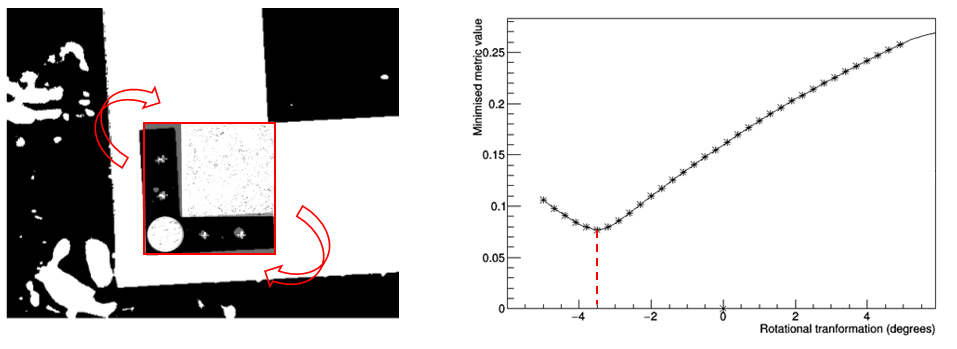
\includegraphics[width=0.9\linewidth]{Data/Control_Software/Template_rotation.png}
\caption{A schematic illustrating the estimation of the sensors planar orientation is shown on the left image. The red arrows indicate the iterative rotational transformations applied to the master image. graph of the minimised metric value versus the angular transformation applied to the master image is shown on the right image. A clear minimum at $\approx$ 3.5 degrees is observed.}
\label{fig:template_rotation}
\end{figure}

\subsection{Location of other corners and extraction of final position and orientation.}
The procedure described in step 2 is repeated at each sensor corner. The planar orientations determined at given corner are used to set the direction of movement needed for the motion stage to automatically travel to an adjacent corner. The final position and orientation of the sensor is determined by a $\chi^{2}$ fit to the four (x,z) points. The orientation determined from the fit is cross-checked with the estimations of the orientation at the corners which accuracy could be not far from $\chi^{2}$ deduced. If there is agreement between the fit and four corner orientations, the fit results are used.

Detailed Flow Chart of the pattern recognition is shown in the Appendix \ref{fig:uml_uml_pattern_recognition}.

\section{Application functionality}

The main window of the application has several buttons and check boxes on top of the window and a number of tabs including: Finder, Threshold, Assembly, Autofocus, Motion Manager and others.

\begin{enumerate}

\item \emph{Finder.} A simple tab the only purpose of each is to show the last acquired image of the camera. This tab also provide a possibility to save current image.

\item \emph{Threshold.} The result of the Threshold operation highly depends on the ambient light thus each new test required threshold value calibration before starting it. This tab is specifically created to control the applying threshold value. It provides the possibility to configure this value and gives an immediate respond by applying Threshold operation on the last acquired image and showing the result under the grayscale original image. The screenshot of the Threshold tab is shown on the Figure \ref{fig:threshold_screenshot}.

\begin{figure}[ht]\centering
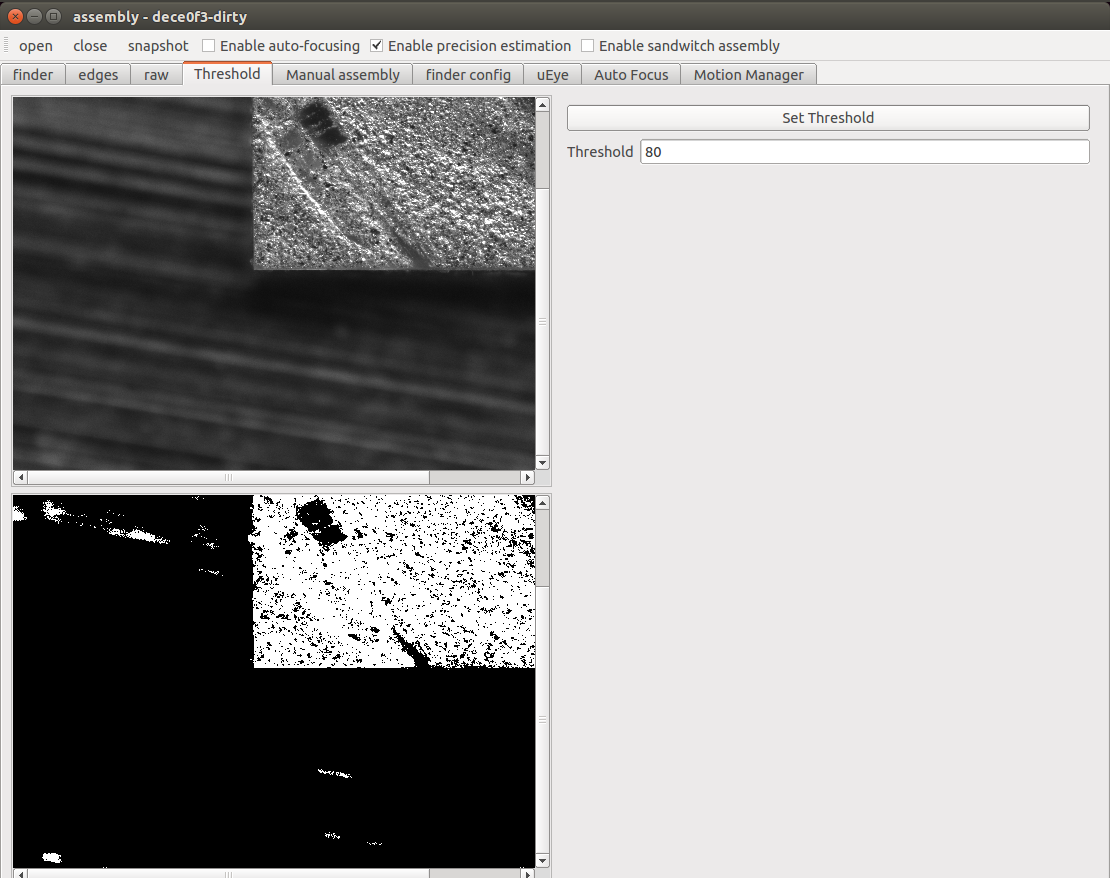
\includegraphics[width=0.7\linewidth]{Data/Control_Software/Threshold_screenshot.png}
\caption{Screenshot of the Threshold tab of the PSAuto application.}
\label{fig:threshold_screenshot}
\end{figure}

\item \emph{Assembly.} The primary tab of the application (Figure \ref{fig:assembly_screenshot}). It contains four image boxes on the left, control tools on the right and motion stage real time status information on the bottom. Left-top image box contains last acquired image. Left-bottom image box -- Thresholded (binary) image of it. Right-bottom image box shows the template image. Finally, right-top image box represents the graph of the last pattern recognition metric distribution of the template matching metric along theta value.

\begin{figure}[ht]\centering
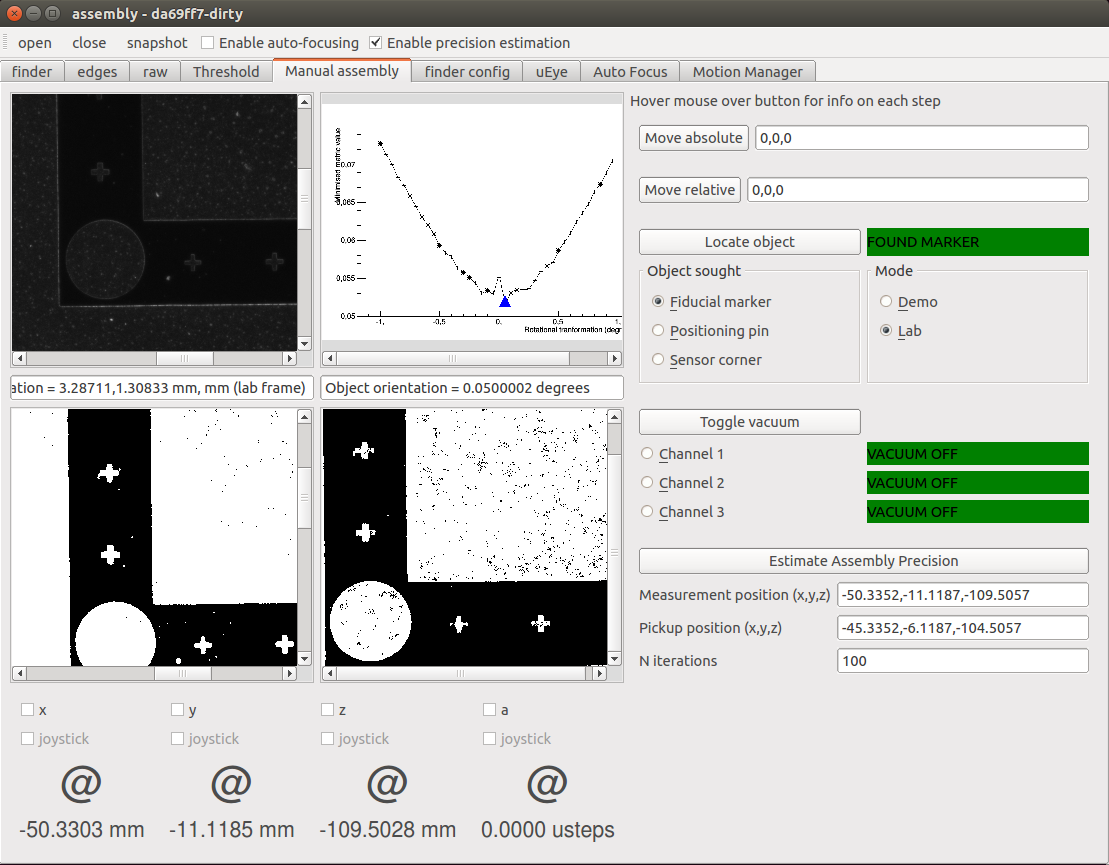
\includegraphics[width=0.7\linewidth]{Data/Control_Software/Assembly_screenshot.png}
\caption{Screenshot of the Assembly tab of the PSAuto application.}
\label{fig:assembly_screenshot}
\end{figure}

On the right side of the tab there are a number of control tools (beginning from the top one):

\begin{itemize}
\setlength\itemsep{-0.5em}
\item Two buttons to move the pickup tool to the absolute or relative position which is written in the forms beside buttons respectively.
\item A set of radio-buttons choosing type of markers on samples and the pattern recognition mode.
\item A set of buttons to control the relay card of vacuum lines. Beside each button there is a real time indicator of the current vacuum line status.
\item The last tool in this tab provides the possibility to conduct tests of the system. It consists of several forms for input test information and a button to start the test.
\end{itemize}

\item \emph{Auto focus.} Another nice tool of the application is autofocus. It place an essential role in the pattern recognition as soon as its accuracy directly depends on the quality of acquired image. There are two features provided by this tab: find the focus position of the camera and move to this position. To find the focus position of the camera it is required to set the step size along Z-axis and the number of steps. As smaller the step is, the more precise focus position will be identified. The idea of auto focus detection is similar to best theta detection in the pattern recognition. For each step position it saves the metric data representing the blur of the acquired image thus in the end the software can find the position with least blur on the image comparing saved metrics for each image.

This algorithm can also be used for another purpose. As soon as the camera is constantly fixed on the robotic arm, it is possible to make relative Z-axis distance measurement. For instance, that can be used for measuring the glue layer thickness of an assembled modules.

\item \emph{Motion Manager.}
This tab provides the control of the motion and rotation stages. Among its functionality are:

\begin{itemize}
\setlength\itemsep{-0.5em}
\item Independent control of X,Y,Z axis and rotation stage.
\item Self-calibration.
\item Real time monitoring of the status of stepper motors of each axis and rotation stage.
\end{itemize}
\end{enumerate}


 % Assembly System

\chapter{Fast adhesive}



\section{Fast glue implementation options}




\section{Candidates}




%\subsection{Two layer Sensors...}


\section{Tests}





\section{Glue joint thickness}





\section{Fast glue conclusions}

 % Fast adhesive

\chapter{Precision estimation tests}
The automated assembly system has a number of properties in terms of precision:
\begin{enumerate}
\setlength\itemsep{-0.5em}
\item Motion stage movement repeatability.
\item Image acquiring repeatability.
\item Precision of pattern recognition.
\item Possible movements of a sensor while picking them up and down with the vacuum pick up tool.
\end{enumerate}

In order to investigate this properties a series of tests were done.
\\Real sensors will be very thin (around 200~um). This fact makes them very fragile. Even though dummy sensors, which will be used for further experiments, is a bit thicker (around 300~um), they are still too fragile for the first tests, because the bottom surface of the pick up tool and the plane underneath testing samples are not yet parallel enough. That is why for the first pick up and down tests we used glass samples. They have the same dimensions and represent close enough the properties of silicon sensors. Moreover, they are much cheaper, so that in case of test failure (sample break) it will not be such a big problem as if silicon sample crashes. Despite all mentioned above, none of glass samples where crashed.
\\Even though we did not do the pick up test with silicon samples, there is still an opportunity to get some information of the pick up and down precision of the silicon samples without direct tests with them. By making a full range of tests with glass samples, we will be able to say how pick up and down influences the precision. Based on this results we will be able to approximately predict the precision of pick up and down tests with silicon samples. Later, when parallelness of the bottom surface of the pick up tool and samples will be provided, we will be able to confirm the results of the prediction.

\section{Pattern recognition precision tests}

For investigation of the pattern recognition precision the following tests were done. During these tests samples were not moved, so that the additional errors by vacuum pick up and down can be excluded.

\subsection{Pattern recognition on the painted corner of a glass dummy}
In the very first test we investigated the pattern recognition on the corner of the sample. Thin pieces of glass with a silver painted corner (Figure \ref{fig:painted_corner}) were used for the tests as an approximation of a silicon sensor. Silver painted corner was used as a marker for pattern recognition to be found in the acquired image.  

\begin{figure}[ht]\centering
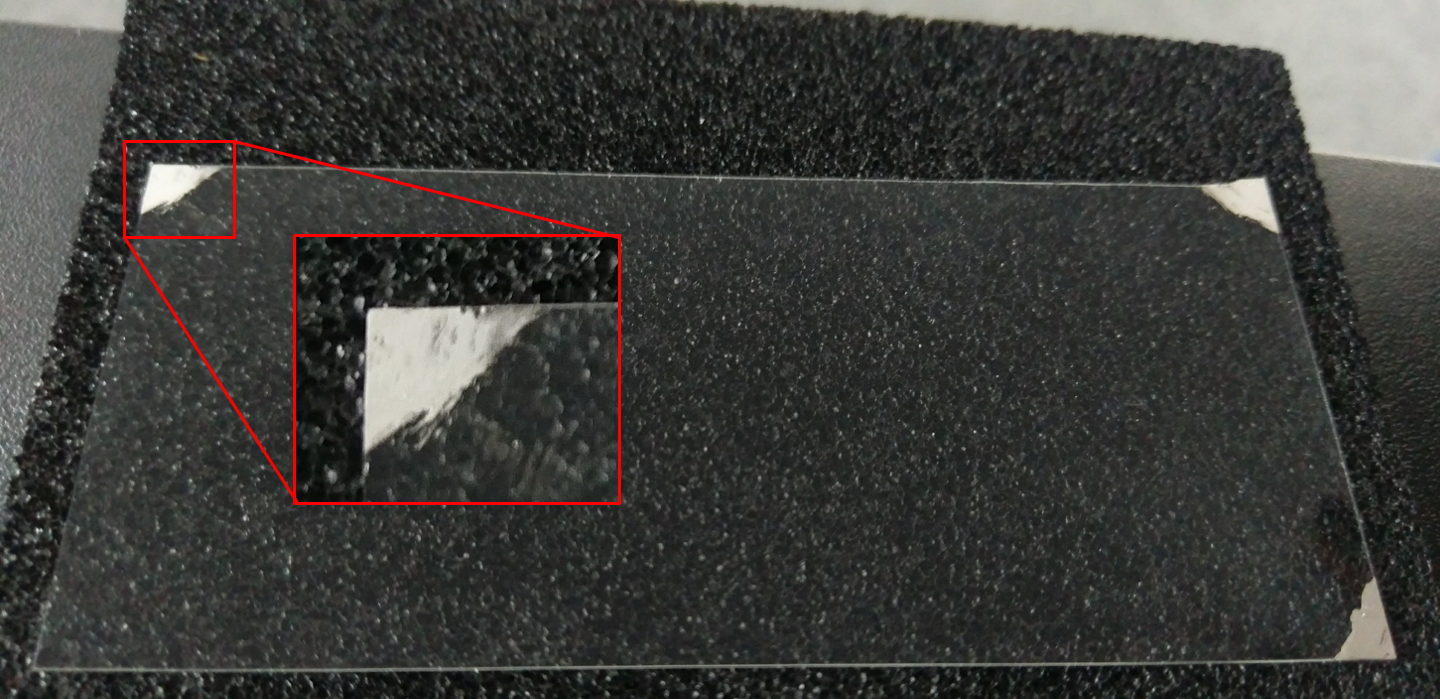
\includegraphics[width=0.8\linewidth]{Data/Precision_tests/Painted_corner.png}
\caption{Glass sample with silver painted corner.}
\label{fig:painted_corner}
\end{figure}

The step-by-step outline of this test is listed below:
\begin{enumerate}
\setlength\itemsep{-0.5em}
\item Move to the image acquiring position.
\item Acquire image and run pattern recognition.
\item Move aside for 5~mm in all three axes.
\item Move to the image acquiring position.
\item Acquire image and run pattern recognition.
\item Save data of the current iteration and go to the next one.
\end{enumerate}

After each step software saves the difference between measured coordinates before and after moving the arm with the camera. The distributions of these values are showed in Figure \ref{fig:corner_x}, Figure \ref{fig:corner_y} and Figure \ref{fig:corner_theta} for X-axis, Y-axis and theta, respectively. The test had 100~iterations done in a row.

\begin{figure}[ht]\centering
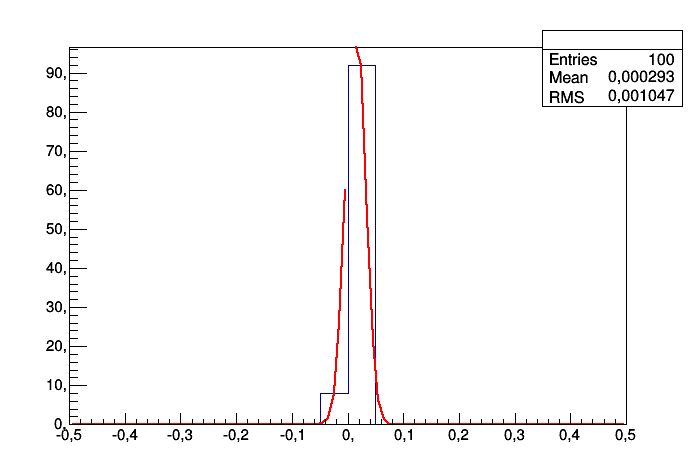
\includegraphics[width=0.8\linewidth]{Data/Precision_tests/Corner_c_x.png}
\caption{Distribution of the difference between detected X coordinate of the master image before and after moving the arm in each iteration. $\Delta X \approx 1~um$. }
\label{fig:corner_x}
\end{figure}

\begin{figure}[ht]\centering
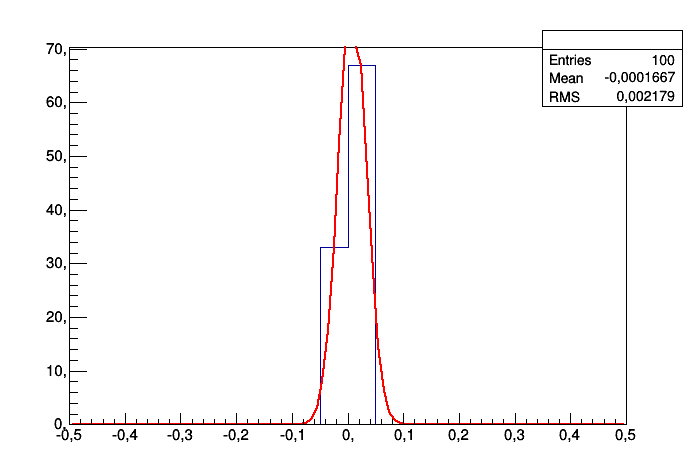
\includegraphics[width=0.8\linewidth]{Data/Precision_tests/Corner_c_y.png}
\caption{Distribution of the difference between detected Y coordinate of the master image before and after moving the arm in each iteration. $\Delta Y \approx 2~um$.}
\label{fig:corner_y}
\end{figure}

\begin{figure}[ht]\centering
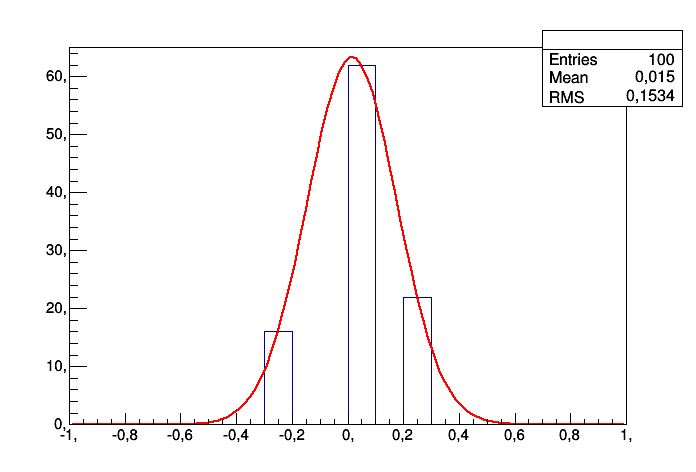
\includegraphics[width=0.8\linewidth]{Data/Precision_tests/Corner_c_theta.png}
\caption{Distribution of the difference between detected angle orientation of the master image relatively to the acquired image before and after moving the arm in each iteration. $\Delta theta \approx 0.15 ~degree$. }
\label{fig:corner_theta}
\end{figure}

Looking at the Figures \ref{fig:corner_x} and \ref{fig:corner_y} one can see that the X, Y detection of the pattern recognition has enough good precision (\underline{1-2~um of error [?]}), while the theta detection results do not look so precise. There are several reasons of such behaviour. The main one them is shown on the Figure \ref{fig:corner_threshold}.

Silver painted surface is not flat in 10~um scale. Due to this roughness different amount of light reflects to the camera from different points along the painted surface. That is why the painted corner contains various shades of grey, which in some points are darker, than the table underneath the sample (background). All these result into the picture one can see in the Figure \ref{fig:corner_threshold}. This kind of pictures has random distribution of dark areas on it. That is why the pattern recognition algorithm has such error while comparing two pictures (master template and acquired image) with random distribution of black areas. Moreover, this kind of tests lasts around one hour, which is long enough for the sun to change the ambient light in the laboratory. Even though all reasonably possible measures were done to prevent such effect, the acquired image is very sensitive for light. For example, the effect of the sun light can results in the threshold variation for 20 units (the color depth is 256) even with covered window in the laboratory.

\begin{figure}[ht]\centering
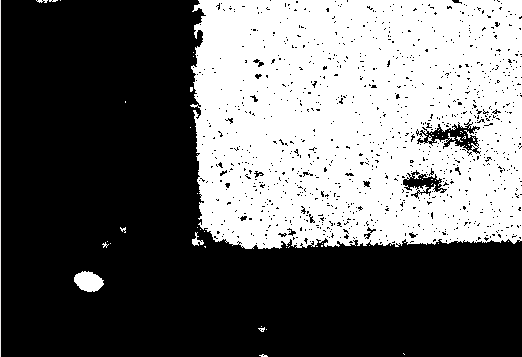
\includegraphics[width=0.8\linewidth]{Data/Precision_tests/Corner_thresholded.png}
\caption{The view of the corner after applying the Threshold.}
\label{fig:corner_threshold}
\end{figure}

\subsection{Pattern recognition on the marker of the dummy sensor}

The same test, but with dummy silicon sensor and real marker on it, was done. Before the test marker was aligned as much close to zero degrees as possible. At the Figure \ref{fig:thresholded_marker} one can see that the edge of the marker after applying Threshold is almost perfect (+/- one pixel). This fact itself is already a proof that Threshold step of pattern recognition is feasible.

\begin{figure}[ht]\centering
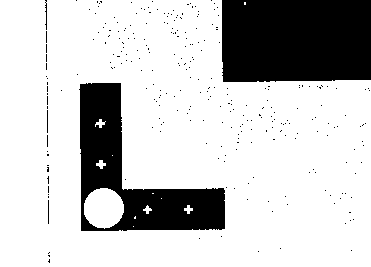
\includegraphics[width=0.6\linewidth]{Data/Precision_tests/Thresholded_marker.png}
\caption{Sensor marker after applying Threshold.}
\label{fig:thresholded_marker}
\end{figure}

The Distribution of X, Y coordinates and theta shows better results than with painted corner, which was expected. For X and Y it is less than a micron, which is already at the limit of camera resolution. $\Delta theta$ is one order of magnitude better than with painted corner --- $\approx 0.02  degree$.

A screenshot of the application during the test is shown on the Figure \ref{fig:zero_peak}. On the pattern recognition curve one can see that at 0 degree there is an unexpected short upward shot. This peak is not a fluctuation and it is not consist of only one point in the plot. As the scale increases, more points form this peak appear. It was not observed in the previous test just because the theta step was one order of magnitude bigger.

\begin{figure}[ht]\centering
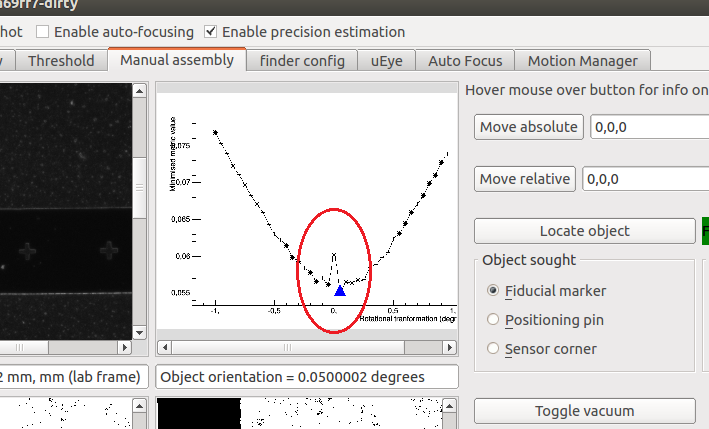
\includegraphics[width=0.8\linewidth]{Data/Precision_tests/Upward_shot.png}
\caption{Screenshot of application during precision estimation test with dummy silicon sensor and marker on it.}
\label{fig:zero_peak}
\end{figure}

\section{Pick-up and -down precision tests}

Next set of tests were oriented to explore the effect of picking-up/down on the precision of the system. In other words, will this process move the sample or not in XY plane. Due to the risk of breaking fragile silicon samples, we used glass ones.

\subsection{Pick-up and -down precision tests without assembly platform}

The first pick-up/down test was done without assembly platform. The step-by-step outline of this test is listed below:
\begin{enumerate}
\setlength\itemsep{-0.5em}
\item Move to the image acquiring position.
\item Acquire image and run pattern recognition.
\item Move to pre-pickup position.
\item Move to pickup position.
\item Turn negative vacuum on.
\item Move up.
\item Move down.
\item Release vacuum.
\item Move down.
\item Move to pre-pickup position.
\item Move to the image acquiring position.
\item Acquire image and run pattern recognition.
\item Save data of the current iteration and go to the next one.
\end{enumerate}

One can notice the step of moving first to pre-pickup position before going to the pick-up position and visa versa. This step is essential. The motion stage provides equal speed in all three axes, so when it receives a command to move to some position it starts to move with equal speed in each of three directions towards the destination simultaneously. As soon as destination in one axis is reached, it obviously stops moving in this axis while moving in other axes is going on. Therefore there is an unlike situation when the robotic arm reaches the sample in Z-axis while X and Y axes would still keep moving, which may cause damage or even break a sample. To prevent such situation we added the step of moving to pre-pickup position.

The results of the test showed movement of the sample, which could be noticed with a naked eye. In order to minimize this movement we decided to make a touch test -- the same as pick-up and -down, but without vacuum. Such kind of test can show the contribution of the touch to the sample movement in the pick-up and -down test. The results if this test was quite similar to the previous test, which means that the touch itself contributes the most to the sample movements in the pick-up and -down test. The interesting fact of this movement is its trend. On Figure \ref{fig:touch_move} one can see X and Y movement trends with respect to iteration number in the touch test. This plots show that the movement is not random and it is more or less constant both in value and direction.

\begin{figure}[ht]\centering
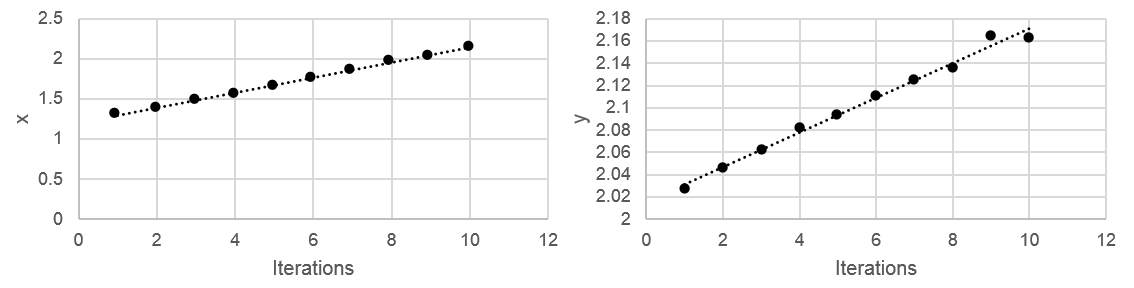
\includegraphics[width=1\linewidth]{Data/Precision_tests/XY_touch_movement.png}
\caption{X and Y movement trends with respect to iteration number in the touch test.}
\label{fig:touch_move}
\end{figure}

The most probable reason for such effect is that pick-up tool surface is not parallel to the table, where samples lay waiting for being picked-up. This fact perfectly corresponds to the constant movement of a sample to the one direction. Unfortunately, it is very complicated to align this surface parallel enough to make sample movement negligible.

\subsection{Pick-up and -down precision tests with assembly platform}

 % Precision Estimation tests

\chapter{Conclusion}



\section{Results}




\section{Future plans}



%\subsection{A Subsection}
 % Conclusion

%\input{Chapters/Chapter6} % Results and Discussion

%\input{Chapters/Chapter7} % Conclusion

%% ----------------------------------------------------------------
% Now begin the Appendices, including them as separate files

\addtocontents{toc}{\vspace{2em}} % Add a gap in the Contents, for aesthetics

\appendix % Cue to tell LaTeX that the following 'chapters' are Appendices

%
\begin{figure}[ht]\centering
\makebox[\textwidth]{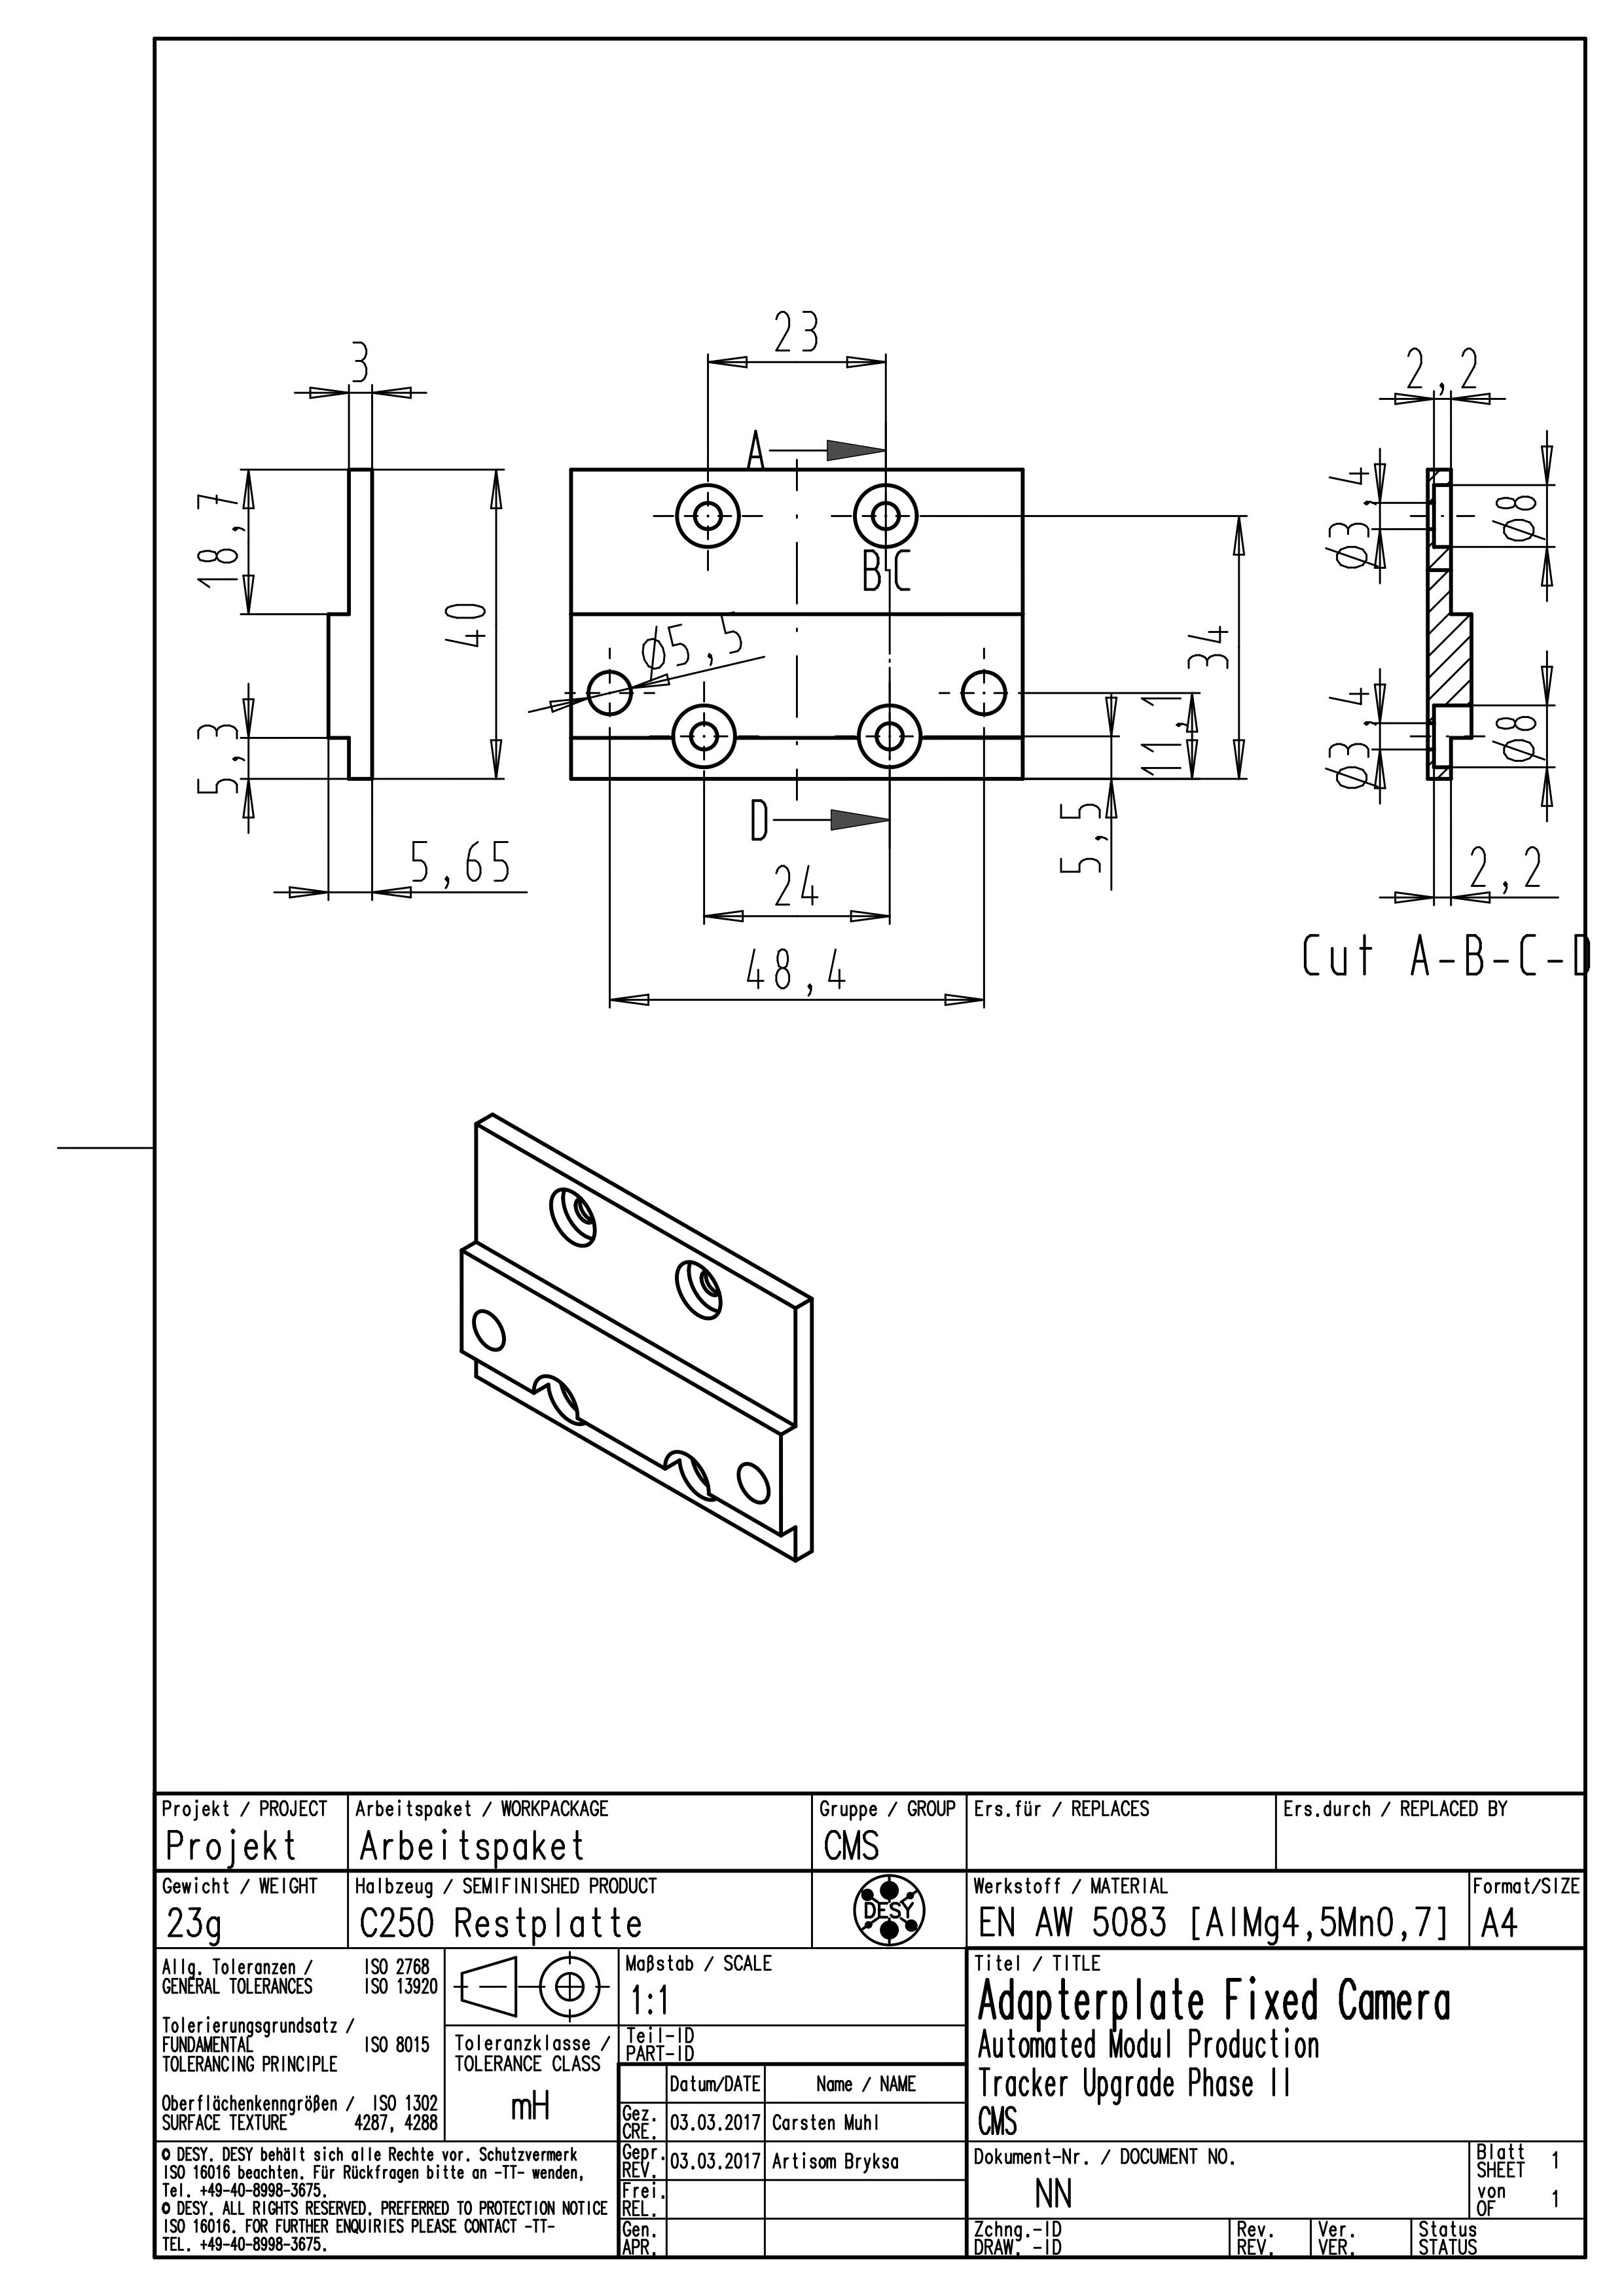
\includegraphics[width=0.8\paperwidth]{Data/Appendices/Adapterplate_Fixed_Camera.png}}
\caption{Prototype of the mechanical jig for module assembly.}
\label{fig:adapter_plate}
\end{figure}

	% Appendix Title

%\input{Appendices/AppendixB} % Appendix Title

%\input{Appendices/AppendixC} % Appendix Title

\addtocontents{toc}{\vspace{2em}}  % Add a gap in the Contents, for aesthetics
\backmatter

%% ----------------------------------------------------------------
\label{Bibliography}
\lhead{\emph{Bibliography}}  % Change the left side page header to "Bibliography"
\bibliographystyle{ieeetr}  % Use the "unsrtnat" BibTeX style for formatting the Bibliography
\bibliography{Bibliography}  % The references (bibliography) information are stored in the file named "Bibliography.bib"

\end{document}  % The End
%% ----------------------------------------------------------------